\section{Lezione del 20 ottobre - Bonizzoni}

Si continua la ricerca di una dimostrazioni di \textbf{NP-completezza}, ambito di studio nato dopo la scoperta di Cook che dimostrava $SAT\in$ \textbf{NP-complete}.\\ 
Ricordiamo:
\begin{itemize}
    \item Se $B$ è un problema tale che $A\leq_p B$, con $A$ \textbf{NP-hard} (o ovviamente anche \textbf{NP-complete}), allora $B$ è \textbf{NP-hard} e se inoltre $B\in NP$ allora $B$ è \textbf{NP-complete}.
    \item Con la transitività della riduzione $\leq_p$ si ha che $\forall\Pi\in NP, \quad \Pi\leq_p A$ e quindi $A$ è \textbf{NP-hard}. Inoltre avendo $A\leq_p B$ ho che  $\Pi\leq_p B$ e quindi $B$ è \textbf{NP-hard}, inoltre, avendo $B\in NP$, ho che è \textbf{NP-complete} 
\end{itemize}   

\subsection{Clique Problem}

Definisco \textbf{clique} (cricca) di un grafo non orientato $G=(V,E)$ come un sottoinsieme $V'\subseteq V$ di vertici tale che: $\forall \,v_1,v_2\in V' (v_1,v_2)\in E$ quindi un sottoinsieme di vertici con solo vertici collegati da un arco.\\
Il \textbf{clique-problem} è un problema di ottimizzazione (nel dettaglio di massimo) in cui si cerca la \textbf{clique} di dimensione massima di un grafo (ovvero $|V'|$ è massimo). Nella versione decisionale chiedo se esiste una \textbf{clique} di dimensione $k$.\\ Il problema \textit{clique} è \textbf{NP-complete}.

\subsubsection{Dimostrazione clique in NP}
Per dimostrare che la \textit{clique} $\in $ NP, per un grafo $G=(V,E)$, usiamo un insieme $V'$ di vertici nella cricca come certificato per l'input $G$. Per verificare che $V'$ è una cricca (dove $V'$ avrà la dimensione pari alla domanda di decisione, ovvero $|V'| = k$) controllerò che $\forall u,v \in V'$, $(u,v) \in E$. Tale verifica è in tempo polinomiale, corrisponde infatti a $\mathcal{O}(|V'| \cdot |V'|)$, ed è quindi quadratico nella dimensione dell'input.

Bisogna ora trovare un problema $A\in {NP-complete}$ tale che $A$ si riduce, in tempo polinomiale, al \textbf{clique-problem} (quindi \textbf{clique-problem} risolve $A$). \\ 
Notiamo che una clique è l'opposto di \textbf{independent-set}, che avevamo dimostrato tramite $3SAT$ (che può risolvere \textbf{independent-set}).\\ 
Quindi per \textbf{clique-problem} provo ancora ad usare $3SAT$. Devo fare in modo che $\phi\in 3SAT$ sse il grafo $G_\phi =(V,E)$ ha una clique di dimensione uguale al numero di clausole di $\phi$. Quindi avendo $k$ clausole in $\phi$ avrò che ciascuna clausola sarà un gadget e da ogni gadget viene preso un singolo vertice che comporrà la clique di dimensione $k$.\\    
Il grafo $G_\phi$ è costruito come nel caso di \textit{independent-set} coi letterali come vertici.\\ Bisogna studiare il collegamento tra tali vertici (che sarà diverso al caso di \textit{independent-set}, non avendo quindi i triangoli).\\

Ipotizzo: 
$\phi=c_1\land c_2\land c_3$ con: $c_1=x_1\lor \neg x_2\lor \neg x_3$, $c_2=\neg x_1\lor x_2\lor x_3$, $c_3=x_1\lor x_2\lor x_3$. \\ 
Per ogni clausola faccio i vertici per ogni letterale (distinti anche per lo stesso letterale, come nel caso di \textit{independent-set}).\\ 
Collego ogni letterale di ogni clausola con ogni altro letterale di ogni altra clausola (non della stessa) a patto che non siano il loro negato, collegando quindi solo vertici \textbf{consistenti}.
\begin{figure}[H]
    \centering
    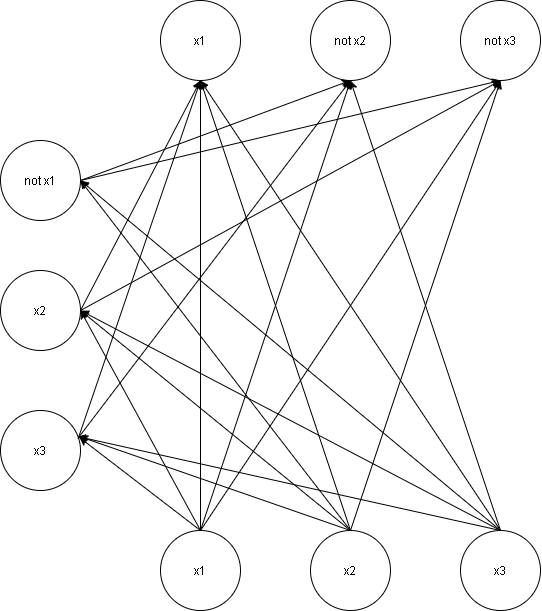
\includegraphics[scale = 0.3]{imm/grafico.png}
\end{figure}

La regola per trasformare $\phi$ nel grafo $G_\phi$, già descritta sopra, la scriviamo ora in modo formale:
\begin{itemize}
    \item per ogni clausola $\displaystyle \in \phi$, $c_r = (l_1^r \lor l_2^r \lor l_3^r $, definiamo un gadget che è un grafo ($G_{c_r}$) che consiste di 3 vertici: $\displaystyle v_1^r \lor v_2^r \lor v_3^r$ in $V$. Dove $\displaystyle V = \bigcup \{v_1^i \lor v_2^i \lor v_3^i\}$, dove però $1 \leq i \leq k$.
    \item $\forall \  v_i^s \lor v_j^r \ \exists $ l'arco $\in E$, sse $l_i^s \lor l_j^r$ sono \textit{consistenti} (il letterale $l_i^s$ non è la negazione di $l_j^r$)
\end{itemize}
Non potrò mai avere più di un letterale per clausola nella clique non essendo tra loro collegati.\\ Passare da $\phi$ a $G_\phi$ ha costo polinomiale in tempo, ottenendo quindi istanza, in tempo polinomiale. \\

Bisogna dimostrare che se $\phi$ ha un assegnamento che la rende vera allora esiste una clique per $G_\phi$ di dimensione $k$. 
Se $\phi$ è vera allora per ogni clausola $c_r$ esiste almeno un letterale che è vero, e assumiamo che tale letterale sia $l_{i}^r = 1$. 
Questo letterale è associato al vertice $v_i^r$ del grafo.Quello che dobbiamo fare è costruire l'insieme dei vertici $V'\subseteq V$ tale che sia formato da quei singoli vertici, $V' = \{ v_i^1, v_j^2 \dots v_z^k\}$, corrispondenti ai singoli letterali veri.  \\ 
L'insieme $V'$ enunciato è una clique, infatti avrò solo letterali collegabili nel grafo, per dimostrarlo dico che $\forall u,v \in V'$, $(u,v) \in E$, ovvero ho solo archi tra letterali consistenti tra loro e quindi, per costruzione, esiste l'arco tra i vertici corrispondenti ($\forall\, u,v\in V'$).\\ 

Inoltre bisogna dimostrare che, se esiste una clique di dimensione $k$, allora $\phi$ è vera e quindi le $K$ clausole sono tutte vere. \\ Per ogni vertice di $v_{it}\in V'$ se appartiene al gadget della clausola $c_t$ rendo vero il letterale associato (o falso se esso è negato). A questo punto rendo vera ogni clausola rendendo vero il letterale associato al vertice della clausola. Da questo so di ottenere un assegnamento di verità per $\phi$ in quanto i letterali sono consistenti. 